\section{Evaluation}
\label{sec:evaluation}
\label{sec:benchmark}

To evaluate the effectiveness of our approach we implemented a variety
of interesting real-life applications including \emph{Numerical
  Differentiation} using the Savitsky-Golay smoothing filter,
\emph{Black Scholes Option Pricing} for pricing European options and
\emph{Ad Prediction} for click-through rate prediction in Microsoft
Bing, but due to lack of space we choose to focus on \emph{Reverse
  Time Migration} (RTM), which is the most complex application in our suite.

RTM is a seismic imaging application used to detect geological
structures, based on the Earth's response to injected acoustic
waves. We used \FAST{} to implement the dataflow kernels for the
memory controllers and the computational kernel.

We used the design space exploration aspect description of Listing
\ref{lst:aspect-exploration} to analyse the trade-offs between
accuracy and resource usage (\Cref{fig:precision}), design scalability
(\Cref{fig:scalability}) and identify resource usage bottlenecks
(\Cref{fig:bottleneck}). This shows that simple aspect descriptions
can be used effectively in the design space exploration process to
identify counter-intuitive results (e.g. the large saving in DSP usage
achieved when decreasing the mantissa from 24 to 22 bits), in a
portable manner. The automated process improves design portability by
allowing optimisations based on design space exploration to be carried
out on various platforms (hence subject to varying resource
constraints) without manual intervention.

\begin{figure}
  \centering
  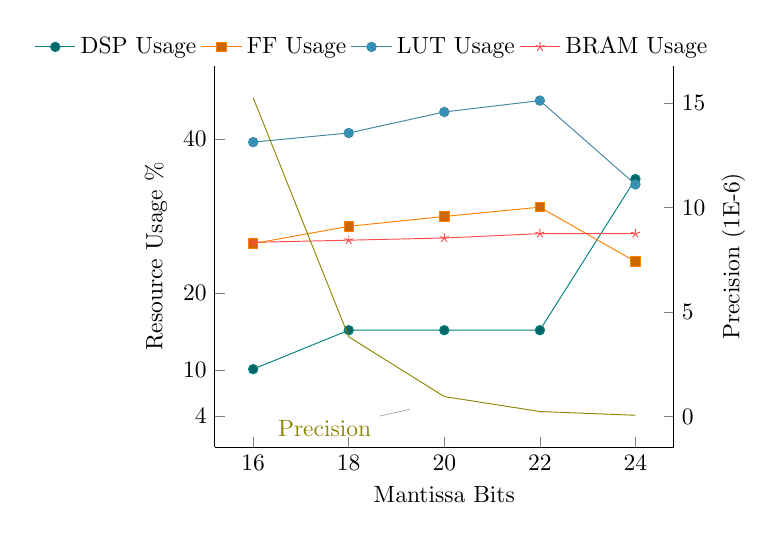
\begin{tikzpicture}[scale=0.85]
    \begin{axis}[
      cycle list name=exotic,
      ymin=0,
      axis y line*=left,
      axis x line*=bottom,
      xlabel=Mantissa Bits,
      ylabel=Resource Usage \%,
      xtick=data,
      ytick={4, 10, 20, 40, 50, 70, 80, 100},
      legend columns=4,
      legend entries={
        DSP Usage,
        FF Usage,
        LUT Usage,
        BRAM Usage},
      legend style={
        draw=none,
        anchor=east,
        at={(1.1, 1.05)}
      }
      ]
      \addplot coordinates {
        (24, 34.82)
        (22, 15.18)
        (20, 15.18)
        (18, 15.18)
        (16, 10.12)
      };
      \addplot coordinates {
        (24, 24.09)
        (22, 31.17)
        (20, 29.96)
        (18, 28.68)
        (16, 26.44)
      };
      \addplot coordinates {
        (24, 34.13)
        (22, 45.02)
        (20, 43.54)
        (18, 40.81)
        (16, 39.62)
      };
      \addplot coordinates {
        (24, 27.73)
        (22, 27.73)
        (20, 27.16)
        (18, 26.88)
        (16, 26.60)
      };
    \end{axis}
    \begin{axis}[
      ylabel=Precision (1E-6),
      axis y line*=right,
      axis x line=none,
      ]
      \addplot[color=olive] coordinates {
        (16, 15.2585)
        (18, 3.8146)
        (20, 0.9536)
        (22, 0.2394)
        (24, 0.0596)
      } node [pos=0.8,pin={190:Precision},inner sep=20pt] {};
    \end{axis}
  \end{tikzpicture}
  \caption{Exploration of accuracy vs resource usage trade-offs using
    the aspect shown in \Cref{lst:aspect-exploration} with variable
    mantissa.}
  \label{fig:precision}
\end{figure}

\begin{comment}
The DSP balancing aspect shown in Listing \ref{lst:aspect-DSP} allows to
explore the resource trade-offs of implementing arithmetic operations
in either DSPs or LUTs and FFs (\Cref{fig:arith}) and helps to
avoid over mapping on DSPs for arithmetic intensive applications.


\begin{figure}[!h]
  \centering
  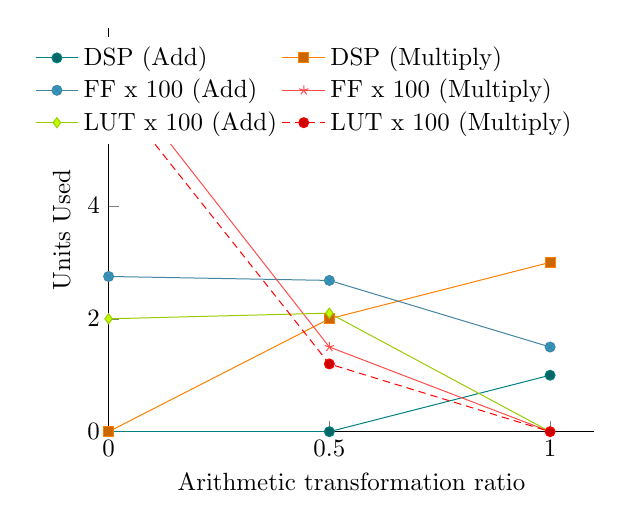
\begin{tikzpicture}[scale=0.9]
    \begin{axis}[
      cycle list name=exotic,
      xmin=0,
      ymin=0,
      axis y line*=left,
      axis x line* =bottom,
      xlabel=Arithmetic transformation ratio,
      ylabel=Units Used,
      xtick={0, 0.5, 1},
      legend columns=2,
      legend entries={
        DSP (Add),
        DSP (Multiply),
        FF x 100 (Add),
        FF x 100 (Multiply),
        LUT x 100 (Add),
        LUT x 100 (Multiply),
      },
      legend style={
        draw=none,
        cells={anchor=west}
      }
      ]
      \addplot coordinates {
        (0, 0)
        (0.5, 0)
        (1, 1)
      };
      \addplot coordinates {
        (0, 0)
        (0.5, 2)
        (1, 3)
      };
      \addplot coordinates {
        (0, 2.75)
        (0.5, 2.68)
        (1, 1.50)
      };
      \addplot coordinates {
        (0, 6.5)
        (0.5, 1.5)
        (1, 0)
      };
      \addplot coordinates {
        (0, 2)
        (0.5, 2.1)
        (1, 0)
      };
      \addplot coordinates {
        (0, 6.13)
        (0.5, 1.2)
        (1, 0)
      };
    \end{axis}
  \end{tikzpicture}
  \caption{Exploration of DSP and LUT/FF balancing for functional units
    implementing a single arithmetic operation using the aspect shown
    in Listing \ref{lst:aspect-DSP}.}
  \label{fig:arith}
\end{figure}


Design space exploration using the aspect in Listing
\ref{lst:aspect-exploration} with increasing parallelism level can be
used to investigate design scalability. For example, for the described
RTM implementation, \Cref{fig:scalability} shows that performance
scales linearly with the number of parallel pipelines and that
significant speedups can be obtained by the \FAST{} dataflow design
compared to the CPU only implementation. Depending on the problem
size, our approach can be used to achieve a significant speedup over
software only versions which is comparable with the best published
FPGA results for static designs
\cite{Xinyu:Qiwei:Luk:Qiang:Pell:2012}, \cite{araya2011assessing}.
\end{comment}

\begin{figure}[!h]
  \centering
  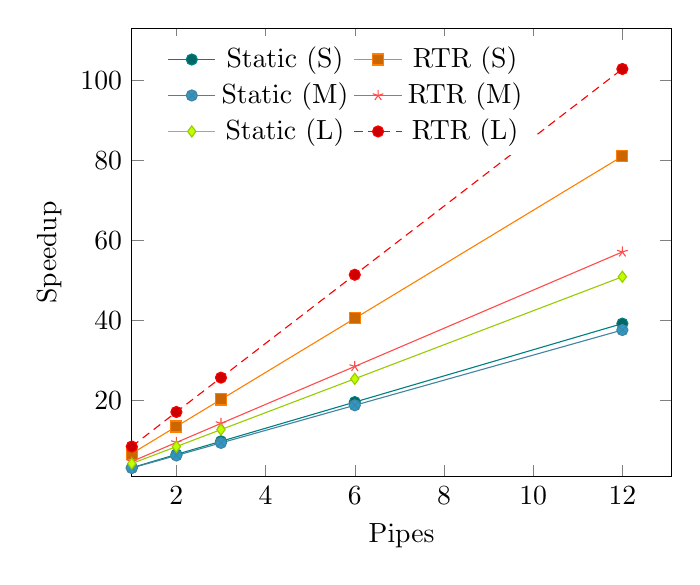
\begin{tikzpicture}
    \begin{axis}[
      cycle list name=exotic,
      xmin=1,
      ymin=1,
      xlabel=Pipes,
      ylabel=Speedup,
      legend columns=2,
      legend entries={
        Static (S),
        RTR (S),
        Static (M),
        RTR (M),
        Static (L),
        RTR (L)},
      legend style={
        draw=none,
        at={(0.05,0.85) },
        anchor=west
      }
      ]
      \addplot coordinates {
        (1, 3.2)
        (2, 6.53)
        (3, 9.8)
        (6, 19.6)
        (12, 39.2)
      };
      \addplot coordinates {
        (1, 6.75)
        (2, 13.5)
        (3, 20.25)
        (6, 40.5)
        (12, 81)
      };
      \addplot coordinates {
        (1, 3.13)
        (2, 6.26)
        (3, 9.4)
        (6, 18.8)
        (12, 37.6)
      };
      \addplot coordinates {
        (1, 4.75)
        (2, 9.51)
        (3, 14.27)
        (6, 28.5)
        (12, 57.1)
      };
      \addplot coordinates {
        (1, 4.25)
        (2, 8.48)
        (3, 12.725)
        (6, 25.42)
        (12, 50.9)
      };
      \addplot coordinates {
        (1, 8.5)
        (2, 17.13)
        (3, 25.7)
        (6, 51.4)
        (12, 102.8)
      };
    \end{axis}
  \end{tikzpicture}
  \caption{Scalability of the RTM dataflow design explored using the aspect
    shown in Listing \ref{lst:aspect-exploration}.}
  \label{fig:scalability}
\end{figure}

\begin{comment}
\Cref{fig:scalability} also shows a model of the performance benefits
of using a run-time reconfigurable implementation generated using the
proposed aspect-oriented approach. Two configurations were created for
the RTM \FAST{} kernel. Since, in our model, during the first half of
the execution time, the backward propagation and imaging functions are
idle, the first configuration requires only half the resources. Hence,
the number of parallel pipelines can be doubled, halving the execution
time of the first configuration. The speedup obtained is comparable to
\cite{Xinyu:Qiwei:Luk:Qiang:Pell:2012}, but the partitioning and
optimisation exploration process is automated via aspects, which
increases developer productivity.
\end{comment}

\begin{figure}
  \centering
  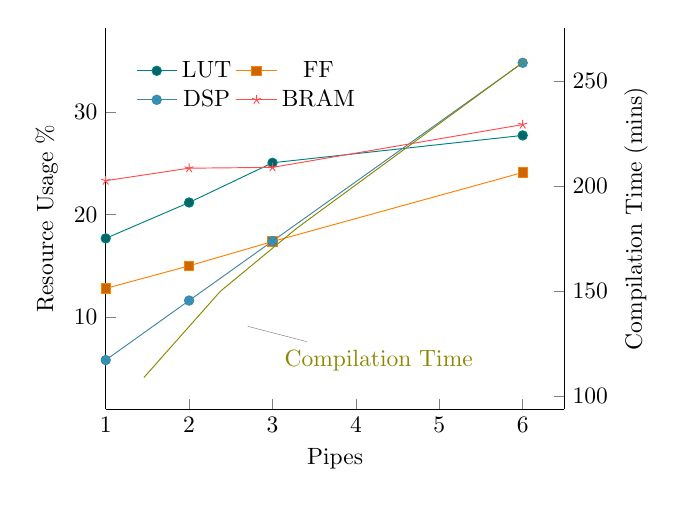
\begin{tikzpicture}[scale=0.85]
    \begin{axis}[
      cycle list name=exotic,
      xmin=1,
      ymin=1,
      xlabel=Pipes,
      ylabel=Resource Usage \%,
      axis x line* =bottom,
      axis y line* = left,
      legend columns=2,
      legend entries={
        LUT,
        FF,
        DSP,
        BRAM,
      },
      legend style={
        draw=none,
        at={(0.05,0.85) },
        anchor=west
      }
      ]
      \addplot coordinates {
        (1, 17.68)
        (2, 21.18)
        (3, 25.06)
        (6, 27.73)
      };
      \addplot coordinates {
        (1, 12.79)
        (2, 15.00)
        (3, 17.37)
        (6, 24.11)
      };
      \addplot coordinates {
        (1, 5.80)
        (2, 11.61)
        (3, 17.41)
        (6, 34.82)
      };
      \addplot coordinates {
        (1, 23.31)
        (2, 24.53)
        (3, 24.61)
        (6, 28.79)
      };
    \end{axis}
    \begin{axis}[
      ylabel=Compilation Time (mins),
      axis y line*=right,
      axis x line=none,
      ]
      \addplot[color=olive] coordinates {
        (1, 109)
        (2, 150)
        (3, 180)
        (6, 260)
      }  node [pos=0.2,pin={340:Compilation Time},inner sep=20pt] {};
    \end{axis}
  \end{tikzpicture}
  \caption{Increase in compilation time and resource usage with number
    of parallel can be used to identify design bottlenecks (limited
    resources which negatively impact design scalability)}
  \label{fig:bottleneck}
\end{figure}

\Cref{table:rtm-performance} compares our implementation using \FAST{}
with other published results and shows that we significantly outperform
CPU implementations in terms of energy efficiency and performance and
match the performance of state-of-the-art manually implemented FPGA
designs.


\begin{table}[!ht]
{\small
  \renewcommand{\arraystretch}{1.5}
  \begin{tabularx}{\linewidth}{c|X|X|X|X|X|X|X|X|X}
    & \textbf{CPU} & \textbf{GPU} \cite{phillips2010implementing} & \textbf{GPU} \cite{datta2008stencil} & \textbf{GPU} \cite{yang2012hybrid}& \textbf{FPGA} \cite{araya2011assessing} & \textbf{FPGA} \cite{Xinyu:Qiwei:Luk:Qiang:Pell:2012} \ & \textbf{FPGA} & \textbf{FPGA D\footnote{D = Dynamic (i.e. using run-time reconfiguration)}} \cite{Xinyu:Qiwei:Luk:Qiang:Pell:2012} & \textbf{FPGA D} \\
    \hline \hline
    Freq.(GHz) & 2.7          & 1.15         &    1.15          &   1.15           &    0.1           & 0.1                 & 0.1                 & 0.1                 & 0.1                 \\
    Time (s)   & 1458         & 52           &    --          &     --         &    --           & 18                  & 18.3                & 13.4                & 13.6                \\
    GFLOP/s    & 0.9          & 51.2         &    36          &     64.5         &    35.8          & 68.0                & 66.8                & 91.6                & 90.2                \\
    Speed-up(X)   & 1           & 56.8        &   40          &     71.6         &     39.7          & 76.4               & \textbf{74.22}     & 102.9              & \textbf{101.3}     \\
    Power (W)  & 185          & --        &    461          &      --        &         --      & 129                 & 126                 & 128                 & 125                 \\
    Efficiency & 4.9          & --        &    78          &       --       &    --           & 527.1               & 527.7               & 715.6               & 721.6               \\
    Eff. Gains & 1           & --        &    15.9          &        --      & --            & 107.5              & \textbf{107.0}     & 146.0             & \textbf{147.1}     \\
  \end{tabularx}
  \caption{Comparison of our RTM implementation with other published results for CPU, GPU and FPGA.}
  \label{table:rtm-performance}
}
\end{table}


Other results from our benchmark suite are summarised in
\Cref{table:benchmark} and show that we can significantly reduce the
number of API calls and lines of code, thus increasing productivity,
while matching performance of manual designs for a wider range of
applications.

\begin{table}
{\small
  \renewcommand{\arraystretch}{1.5}
  \begin{tabularx}{\linewidth}{X|X|X|X|X|X}
    \textbf{Kernel} & \textbf{Size} & \textbf{Reduction} & \textbf{API Calls} & \textbf{Performance}              & \textbf{Resource}
    \\
    \hline\hline
    CmdRead       & 48 & 43 \%               & 4.33                     & \multirow{2}{1.5cm}{$ > 75\%$}        & \multirow{6}{1.5cm}{$\approx 100\%$} \\
    CmdWrite      & 54  & 31 \%              & 4.13                     &                                   &                              \\
    \cline{1-4}
    RTM            & 231 & 27 \%              & 10                       & \multirow{5}{1.5cm}{$ \approx 100\%$} &                              \\
    SGSmooth      & 60 & 45 \%              & 14                       &                                   &                              \\
    SGDiff       & 58 & 42 \%              & 14                       &                                   &                              \\
    Black-Scholes & 56  & 60 \%               & 5.5                      &                                   &                              \\
    \cline{5-5}
    Ad Prediction & 94 & 40 \%             & 16                       &                                   &    $ \approx 117 \% $                          \\
    Bitonic Sort & 102 & 38 \%             & 12                    &                                   &    $ \approx 100 \% $                          \\
  \end{tabularx}
  \caption{Lines of code, API calls performance and resource usage ratio of original manual MaxCompiler design and \FAST{} design.}
  \label{table:benchmark}
}
\end{table}

\begin{comment}
  \section{Numerical Differentiation}

  Numerical differentiation is an important application in engineering
  and can be used to estimate derivative values when an analytical form
  of the function is not available. Consider for example the case of
  measuring a sample of displacements form which we want to derive the
  instantaneous speed. As explained in \Cref{sec:num-diff-back} a 5
  point linear stencil can be used to approximate the value of the
  derivative.

  However, in practice, experimental data often contains noise (unwanted
  random addition to a signal) which impacts the accuracy of the
  estimation. To filter the noise, a smoothing step is applied to the
  experimental data with the goal of improving the signal-to-noise
  ratio. One of the most commonly used examples is the Savitzky-Golay
  Filter \cite{savitzky1964smoothing} which applies a polynomial
  regression to a set of a m data points, also a linear stencil
  computation.  Using higher order stencils (up to a few hundreds even)
  results in an smoother, less noisy regression.

  Hence our implementation of the differentiation algorithm consists of
  two steps: \emph{1)} applying the smoothing filter to the input data,
  \emph{2)} estimating the derivative using a linear stencil. The
  algorithm for an arbitrary stencil order is shown in Algorithm
  \ref{alg:sg-numdiff}.

  \begin{algorithm}
    \caption{Savitzky-Golay Numerical Differentiation}
    \label{alg:sg-numdiff}
    \begin{algorithmic}
      \Function{NumericalDifferentiation}{$values, Order, sCoefs, dCoefs, sn, dn, Step$}
      \State smoothValues $\gets$ \Call{Convolve}{$values, sCoefs, Order, sn$}
      \State diffValues  $\gets$ \Call{Convolve}{$values, dCoefs, Order, dn * step$}
      \State \Return $diffValues$
      \EndFunction

      \Function{Convolve}{$values, coeffs, Order, Normalizer$}
      \State result[] $\gets$ 0
      \For{$x = Order \to (nCoefs - Order)$}
      \For{$c = 1 \to nCoefs$}
      \State result[x] $\gets$ result[x] + value[x - Order + c] * coeffs[c]
      \EndFor
      \State result[x] $\gets$ result[x] / Normalizer
      \EndFor
      \State \Return result
      \EndFunction
    \end{algorithmic}
  \end{algorithm}

  Our \FAST{} dataflow designs consist of two kernels one for smoothing
  and one for differentiation. We explore the possibility of generating
  an efficient run-time reconfigurable design either for improving
  design performance, or for supporting larger dimension stencils, via
  time-sharing. We measure resource usage and performance for stencil
  size of 5, 7 and 9 points and estimate the resource usage for larger
  stencils to identify sizes at which run-time reconfiguration becomes
  convenient. To maximise performance we write a parametrised design
  which can be parallelised up to the point where it becomes memory
  bound.

  Since the design uses PCI-E the maximum parallelism that can be
  achieved before it becomes I/O bound is given by:
  $$\frac{\text{PCI-E bits per cycle}}{\text{kernel input bits}} = \frac{128}{32} = 4$$

  Hence, when using PCI-E a kernel replication factor of 4 is ideal for
  maximising throughput.

  If data were available straight from FPGA DRAM the design parallelism
  could be increased to:
  $$\frac{\text{memory bits per cycle}}{\text{kernel input bits}} = \frac{1536}{32} = 48$$

  However, for this algorithm transferring data to on-board DRAM will
  not improve overall throughput since data are only used once, hence we
  investigate the PCI-E design.

  The measured resource usage scales linearly with the parallelism level
  as shown in \Cref{table:nd1} and shows that for a 7 point stencil,
  approximately 10 pipelines can mapped onto the FPGA. However, beyond
  80\% resource usage level, the design usually becomes fairly congested
  and fails to route or takes an extremely large time to achieve timing
  closure.

  \begin{table}[ht!]
    \begin{tabularx}{\textwidth}{X|X|X|X|X}
      Pipes & LUT Usage & FF Usage & DSP Usage & BRAM Usage \\
      \hline\hline
      1     & 10.01     & 6.65     & 8.45      & 0.75       \\
      2     & 18.91     & 13.21    & 17.51     & 1.50       \\
      4     & 37.13     & 25.32    & 33.12     & 3.75       \\
      6     & 56.17     & 39.28    & 50.31     & 4.50       \\
      8     & 79.63     & 51.22    & 49.55     & 7.75       \\
    \end{tabularx}
    \caption{Pipeline scalability of the numerical differentiation algorithm for a 7 point stencil.}
    \label{table:nd1}
  \end{table}

  \Cref{table:nd2} shows that the maximum achievable stencil width with
  the static design (which uses both kernels onto the FPGA chip) is 29
  whereas using run-time reconfiguration to swap the individual kernels
  increases the maximum stencil width to around 59 points (computed an
  assumed 4 parallel pipelines as shown on lines 4, 8 and 9 of
  \Cref{table:nd2}).

  \begin{table}[ht!]
    \begin{tabularx}{\textwidth}{X|X|X|X|X|X}
      Kernel                    & Stencil Width & LUT Usage & FF Usage & DSP Usage & BRAM Usage   \\
      \hline\hline
      \multirow{4}{*}{GSDiff}   & 5             & 2.03      & 1.55     & 0.99      & 0            \\
      & 7             & 2.79      & 2.08     & 2.92      &              \\
      & 9             & 3.33      & 2.48     & 3.76      & 0            \\
      \cline{2-6}
      & \multicolumn{5}{c}{Max = $100 / 3.76 * 9 / 4 = 239 / 4 = 59 $} \\
      \hline
      \multirow{4}{*}{GSSmooth} & 5             & 2.34      & 1.44     & 2.23      & 0            \\
      & 7             & 2.91      & 1.81     & 2.97      & 0            \\
      & 9             & 3.47      & 2.21     & 3.91      & 0            \\
      \cline{2-6}
      & \multicolumn{5}{c}{Max = $100 / 3.91 * 9 / 4 = 239 / 4 = 57 $} \\
      \hline
      Both                       & \multicolumn{5}{c}{Max = $100 / (3.91 + 3.76) * 9 / 4 = 29 $}  \\
    \end{tabularx}
    \caption{Resource usage per stencil width, per kernel, per compute pipe.}
    \label{table:nd2}
  \end{table}


  The \FAST{} dataflow kernel that implements the differentiation
  operation is shown in \Cref{app:numdiff}. It uses no API (non-user
  defined) function calls and a total of 20 lines of code, compared to
  the original MaxCompiler design which requires 14 API calls and 37
  lines of code.

  \section{Black Scholes}

  The finite difference implementation for the Black Scholes
  application is interesting since it introduces an element
  characteristic to stencil computations and also to designs that
  perform well on the Maxeler platform: multiple time step
  iteration. This enables and requires local data reuse via on-board
  DRAM to achieve maximum performance. This is because the PCI-E bus
  can only provide a maximum bandwidth of 2GB/s whereas DRAM achieves a
  maximum of 38GB/s.

  The \FAST{} kernel for the Black Scholes finite difference kernel was
  introduced in \Cref{sec:fast-ref}. The DRAM command read generator is
  shown in Listing \ref{mem-ctl}. This requires a more complicated
  chain counter structure (where one counter is only enabled when its
  child in the chain is just about to wrap to zero) in order to control
  the memory access pattern. Additionally, a call to \texttt{DRAMOutput}
  is required to send the memory commands to the appropriate stream
  controller. For this reason, this kernel is an example where our
  approach is not very effective at reducing code size or number of API
  calls. Still, the equivalent MaxCompiler design shown in
  \Cref{app:mem-read-kernel} requires 23 API calls and 19 lines of
  code, compared to 3 API calls and 13 lines of code required in \FAST{}.

  \begin{lstlisting}[caption={\FAST{} Memory Controller Kernel}, label={mem-ctl}]
    #include "fastc/fast.h"

    void kernel_Cmdread(unsigned int iniBursts, unsigned int totalBursts,
    unsigned int wordsPerBurst, bool Enable)
    {
      int wordCount = count_p(32, wordsPerBurst, 1, Enable);
      int* wrap;
      *wrap = (wordCount == wordsPerBurst - 1) & Enable;
      int burstCount = count_p(32, totalBursts, Burst_inc, wrap);
      int *Control;
      *Control = (wordCount == 0) & Enable;
      DRAMOutput("dram_read", Control,
      burstCount + iniBursts,
      Burst_inc, 1, 0, 0);
    }

  \end{lstlisting}

  Design space exploration using the iterative design exploration
  aspect shows that the design can easily fit up to 60 parallel
  processing pipelines. However the \Cref{fig:bscoles-exp} shows that
  the maximum measured parallelism is 48, since after this point the
  kernel becomes I/O bound even with DRAM.

  \begin{figure}[!h]
    \centering
    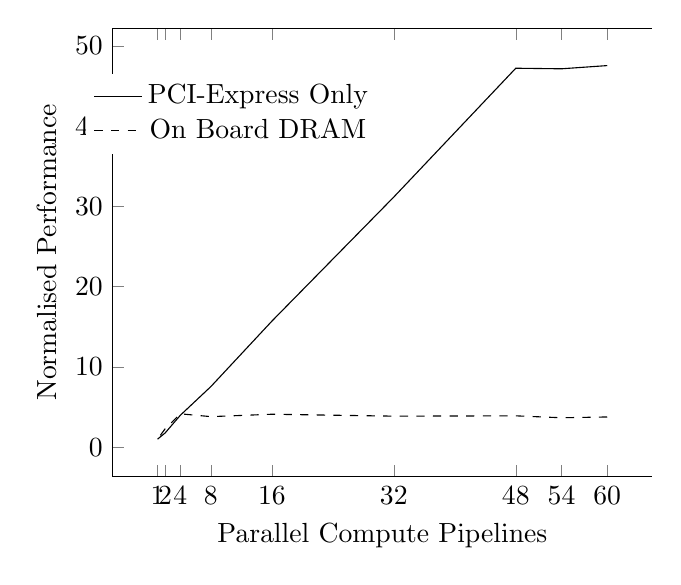
\begin{tikzpicture}
      \selectcolormodel{gray}
      \begin{axis}[
        axis y line*=left,
        xlabel=Parallel Compute Pipelines,
        ylabel=Normalised Performance,
        xtick=data,
        legend columns=1,
        legend entries={
          PCI-Express Only,
          On Board DRAM
        },
        legend style={
          draw=none,
          at={(0.5, 0.9)}
        }
        ]
        \addplot[solid] coordinates {
          (60, 47.56)
          (54, 47.16)
          (48, 47.23)
          (32, 31.18)
          (16, 15.71)
          (8, 7.56)
          (4, 3.99)
          (2, 1.78)
          (1, 1)
        };
        \addplot[dashed] coordinates {
          (60, 3.77)
          (54, 3.67)
          (48, 3.91)
          (32, 3.87)
          (16, 4.11)
          (8, 3.81)
          (4, 4.16)
          (2, 2.3)
          (1, 1)
        };
      \end{axis}
    \end{tikzpicture}
    \caption{Bandwidth / computation ratio exploration using the
      iterative exploration aspect description.}
    \label{fig:bscoles-exp}
  \end{figure}




  \section{Reverse Time Migration}
  \label{sec:RTM}

  \section{Bitonic Sort}

  Sorting networks \cite{batcher1968sorting} are an interesting
  benchmark application for our approach since it is both an important
  application but also fairly challenging to fit into the proposed
  programming model:
  \begin{itemize}
  \item Sorting networks constitute the basic blocks for
    high-performance multi-gigabyte sorting which in the context of the
    HARNESS project, is an important case study for key cloud
    applications;
  \item Sorting networks are not easily mapped to FPGA since resource
    constraints limited considerably the input size of the network; for
    example, our sorting network implementation fails to achieve timing
    closure
  \item Comparison based sorting requires very little arithmetic, which
    is a major disadvantage on the Maxeler Platform, since DSPs cannot
    be utilised
  \item Sorting in general is an application that does not map well onto
    the streaming model of computation, since due to the aforementioned
    resource constraints, merging of buckets of values is required which
    leads to a feed-back loop in the design;
  \end{itemize}

  We implement a bitonic sorting network for inputs of $n$ arrays of
  size $k = (4, 8, 32, 64, 128, 256)$ elements. We compare the
  performance of the design with the ANSI C implementation of
  \texttt{qsort()}
  \footnote{http://www.umcs.maine.edu/~chaw/200801/capstone/n/qsort.c}
  which is a hybrid of insertion-sort and quicksort. For a fixed network
  size, we vary the input size to compare the software and hardware
  implementations and report the average results of 50 runs.

  The implemented sorting network has the following properties:
  \begin{itemize}
  \item $\text{complexity} = \text{network depth} = \frac{n * log(n)}{2} = O(log^2(n))  $
  \item $\text{comparators} = n * log(n) * (log(n) + 1) / 4 = O(n * log^2(n)) $
  \end{itemize}

  Execution results are depicted in \Cref{fig:bsort-scalab} (experimental
  data is shown in \Cref{app:experimental-data}) and show that the
  hardware version outperforms the software version for values of n
  larger than $2^{14}$ with speedups increasing from 1.25X to 24X, in
  proportion with the value of n and also depending on the network input
  width. Thus higher speedups can be obtained for large network sizes,
  providing the incentive for adaptive run-time reconfiguration, based
  on the observed range of input values, at run-time. Although the
  compute only speedup is significant even for smaller values of $n$ the
  execution time is dominated by the overhead of data transfer over
  PCI-Express from main memory to the FPGA accelerator.

  \begin{figure}[!ht]
    \centering
    \hspace{-1cm}
    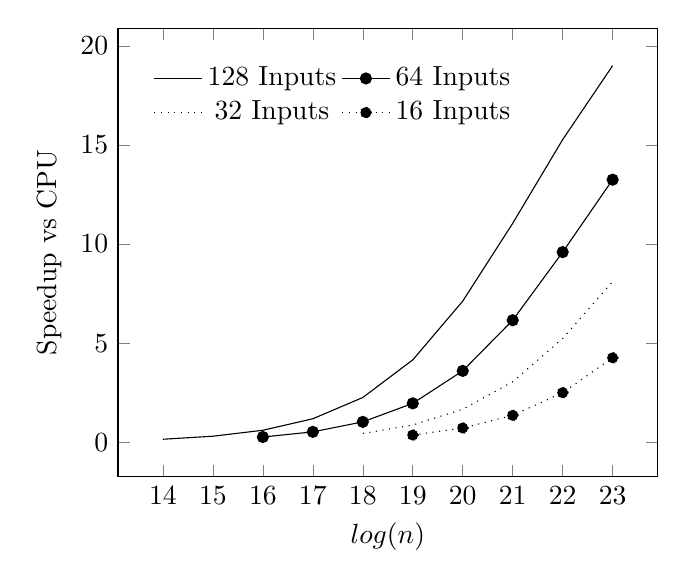
\begin{tikzpicture}
      \begin{axis}[
        ylabel=Speedup vs CPU,
        xlabel=$log(n)$,
        xtick=data,
        legend columns=2,
        legend entries={
          128 Inputs,
          64 Inputs,
          32 Inputs,
          16 Inputs
        },
        legend style={
          draw=none,
          at={(0.05,0.85) },
          anchor=west
        }
        ]
        \addplot[mark=none] coordinates {
          (14, 0.1551)
          (15, 0.3084)
          (16, 0.6084)
          (17, 1.1881)
          (18, 2.26)
          (19, 4.1585)
          (20, 7.1215)
          (21, 11.0465)
          (22, 15.2691)
          (23, 18.9995)
        };
        \addplot[mark=*] coordinates {
          (16, 0.2677)
          (17, 0.5274)
          (18, 1.0317)
          (19, 1.9652)
          (20, 3.6039)
          (21, 6.1588)
          (22, 9.594)
          (23, 13.2481)
        };
        \addplot[dotted] coordinates {
          (18, 0.4467)
          (19, 0.8722)
          (20, 1.6663)
          (21, 3.0527)
          (22, 5.237)
          (23, 8.1093)
        };
        \addplot[mark=*, dotted] coordinates {
          (19, 0.3664)
          (20, 0.7221)
          (21, 1.3596)
          (22, 2.5036)
          (23, 4.2621)
        };
      \end{axis}
    \end{tikzpicture}
    \caption{Speedup vs CPU of the bitonic sorting network designs for
      large batches of small inputs.}
    \label{fig:bsort-scalab}
  \end{figure}

  Given that execution time is dominated by the transfer time,
  reconfiguring the design to increase parallelism will bring a small
  performance benefit.  The situation changes when the network is used
  as part of a general purpose sorting algorithm. The complexity $(
  O(N/k * logn * log(n/k)) $ decreases linearly with the increase in the
  network width. This would provide the motivation to adapt the network
  to input patterns, switching to larger networks for small observed
  values. One factor to consider is that, reducing to smaller network
  sizes can also decrease the communication overhead. Since all network
  inputs must be present, additional padding is required for arrays that
  are not of a length which is a power of two.

  Hence it is only necessary to reconfigure when a change in the input
  pattern is detected that requires smaller computational ranges of
  values. Results of exploring maximum word length using the iterative
  design space exploration aspect description show that decreasing word
  width and varying the type (floating or fixed point, based on the
  input characteristics) allow us to build larger network sizes, which
  are capable of substantially higher throughput. Since throughput
  increases linearly with the networks size, reconfiguring the FPGA to
  adapt to smaller data representations can more than double the
  performance of networks for small input values. The maximum network
  size is determined by iteratively increasing network width until the
  design overmaps or fails to meet timing at the next iteration (columns
  6 and 7 of \Cref{table:bsort-bitwidth}).

  \begin{table}[!ht]
    \begin{tabularx}{\textwidth}{X | X | X | X | X | p{2cm} |  X}
      \textbf{Type} & \textbf{Width} & \textbf{Max. Size} & \textbf{LUT \%} & \textbf{FF \%} & \textbf{Overmaps} & \textbf{Meets Timing} \\
      \hline
      \hline
      int           & 32             & 128                & 42.87           & 43.75          & yes               & no                    \\
      int           & 16             & 128                & 42.87           & 43.75          & no                & no                    \\
      int           & 8              & 256                & 32.06           & 31.62          & no                & no                    \\
      float         & (8, 24)        & 64                 & 34.19           & 18.12          & yes               & no                    \\
      fixed         & (8, 24)        & 128                & 42.79           & 43.75          & yes               & no                    \\
      fixed         & (24, 8)        & 128                & 42.79           & 43.75          & yes               & no                    \\
    \end{tabularx}
    \caption{Results of exploring different network sizes and data types for the bitonic sorting network}
    \label{table:bsort-bitwidth}
  \end{table}


  \section{Ad Prediction}

  The Ad prediction kernel implemented for this benchmark application
  was proposed for predicting click-through rate for sponsored search on
  the Bing search engine \cite{graepel2010web}. Given as input the prior
  probability for a number of features, Bayesian inference is used to
  determine the posterior probability. The values of features are
  arbitrarily large (so fixed point optimisations cannot be used) and
  prediction accuracy increases with number of features considered by
  the algorithm. Increasing the number of features results in
  replicating most of the computational pipeline and additional levels
  being added to the adder tree that reduces the results. It is an
  interesting application because it makes use of expensive arithmetic
  operations such as exponentiation and square root. The original
  MaxCompiler implementation was developed as part of the HARNESS
  validation studies. Additionally, helper functions require function in
  lining. The results of the design space exploration show that this is
  a particularly challenging application to map onto the FPGA and
  requires ability to tune floating point mantissa. This makes use of
  our pragma for specifying stream I/O and compute type.

  The \FAST{} dataflow implementation is shown in
  \Cref{app:add-prediction}.  The total number of lines of code for the
  Ad Prediction kernel is 67 and the kernel requires 3 API calls. The
  original MaxCompiler design has 90 lines of code and 49 API calls.


  The iterative exploration aspect description and the operator
  optimisation aspect can be used for design space exploration to vary
  the number of features of the algorithm and the DSP mapping factor to
  achieve timing closure.

  \Cref{table:adp-dse} shows the parameters used for design space
  exploration to achieve timing closure. The ability to map operations
  from LUT/FFs to DSP enables the design space exploration process to
  achieve timing closure.
  \begin{table}
    \renewcommand{\arraystretch}{1.2}
    \begin{tabularx}{\textwidth}{X|X|X|X}
      \textbf{Features} & \textbf{DSP Factor} & \textbf{Representation} & \textbf{Meets Timing} \\
      \hline \hline
      10        & Full       & float(8, 24)   & No           \\
      10        & Balanced   & float(8, 24)   & No           \\
      10        & Zero       & float(8, 24)   & No           \\
      10        & None       & float(8, 16)   & No           \\
      10        & None       & float(8, 10)   & No          \\
      10        & Full       & float(8, 10)   & Yes          \\
      8         & None       & float(8, 24)   & No           \\
      8         & Full       & float(8, 24)   & No           \\
      8         & Balanced   & float(8, 24)   & No           \\
      4         & Full       & float(8, 24)   & Yes          \\
      4         & Balanced   & float(8, 24)   & Yes          \\
      4         & Full       & float(8, 16)   & Yes          \\
      4         & Full       & float(8, 10)   & Yes          \\
      2         & None       & float(8, 24)   & Yes          \\
      2         & Balanced   & float(8, 24 )  & Yes          \\
      2         & Full       & float(8, 24)   & Yes          \\

    \end{tabularx}
    \caption{Design exploration space for the Ad Prediction kernel.}
    \label{table:adp-dse}
  \end{table}

  \section{Summary}

  We have analysed our implementation on a number of real-life
  applications. Table{conc:summary} summarises our experimental results
  and shows that for the considered applications we can achieve close to
  identical performance to hand crafted MaxCompiler designs, while
  requiring significantly less line of code and API calls even without
  taking into account savings that can be achieved from using aspect
  descriptions.




  Our extensions for multiple kernel support and supporting designs with
  DRAM has helped match the performance of MaxCompiler designs that
  benefit from higher memory bandwidth (such as Black Scholes or
  RTM). In the meantime the ability to infer types has helped simplify
  the language reducing the number of API calls substantially. The
  aspect oriented design flow can be used to effectively explore the
  design space of available optimisation for operand bit width, or
  varying specific design constants in order to achieve timing closure
  or maximise performance. Although these results are promising, it must
  be noted that these metrics alone are not a definitive indication of
  increased productivity and that future large scale studies should be
  performed.

  One limitation of our current implementation is that we cannot control
  design parameters that are not directly accessible to the dataflow
  kernel. For example stream clock frequency and DRAM frequency are
  controlled from within the MaxCompiler manager. To work around this
  limitation for evaluation purposes we have reproduced the same manager
  design in both the original MaxCompiler design and the \FAST{} design
  when measuring performance.
\end{comment}